% the rings 1 to 20 of the nuclear spine, opened into their measured isotopes (AME2020)
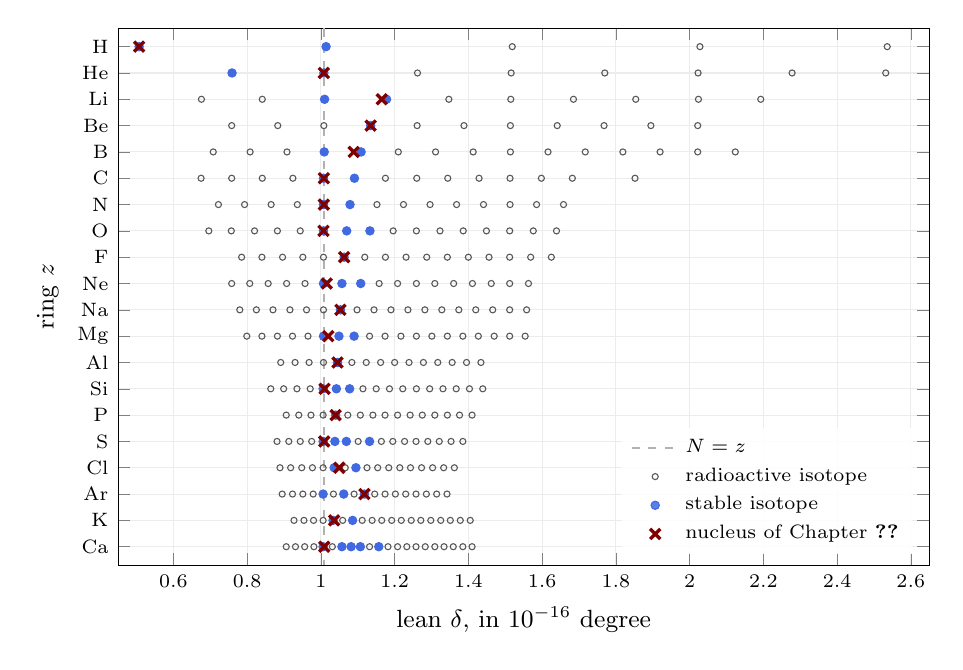
\begin{tikzpicture}
\begin{axis}[width=0.98\textwidth, height=8.4cm, y dir=reverse,
  xmin=0.45, xmax=2.65, ymin=0.3, ymax=20.7, ytick={1,2,...,20}, yticklabels={H,He,Li,Be,B,C,N,O,F,Ne,Na,Mg,Al,Si,P,S,Cl,Ar,K,Ca},
  xlabel={lean $\delta$, in $10^{-16}$ degree}, ylabel={ring $z$},
  tick label style={font=\scriptsize}, label style={font=\small}, grid=major, grid style={gray!15},
  legend style={font=\scriptsize, draw=none, fill=white, fill opacity=0.85, text opacity=1, at={(0.98,0.02)}, anchor=south east}, legend cell align=left]
\addplot[gray!60, dashed, thick] coordinates {(1.00748,0.3) (1.00748,20.7)};\addlegendentry{$N = z$}
\addplot[only marks, mark=o, mark size=1.1pt, gray!70!black] coordinates {(1.519,1.000) (2.028,1.000) (0.676,3.000) (2.536,1.000) (1.262,2.000) (0.841,3.000) (3.045,1.000) (1.516,2.000) (0.758,4.000) (1.770,2.000) (0.883,4.000) (0.708,5.000) (2.023,2.000) (1.347,3.000) (1.008,4.000) (0.808,5.000) (0.675,6.000) (2.278,2.000) (1.515,3.000) (0.908,5.000) (0.758,6.000) (2.532,2.000) (1.685,3.000) (1.261,4.000) (0.841,6.000) (0.722,7.000) (1.854,3.000) (1.388,4.000) (0.924,6.000) (0.793,7.000) (0.696,8.000) (2.024,3.000) (1.514,4.000) (1.210,5.000) (0.865,7.000) (0.757,8.000) (2.193,3.000) (1.641,4.000) (1.311,5.000) (0.936,7.000) (0.820,8.000) (1.768,4.000) (1.413,5.000) (1.175,6.000) (0.882,8.000) (0.785,9.000) (1.895,4.000) (1.514,5.000) (1.260,6.000) (0.944,8.000) (0.840,9.000) (0.758,10.000) (2.022,4.000) (1.616,5.000) (1.344,6.000) (1.152,7.000) (0.896,9.000) (0.807,10.000) (1.717,5.000) (1.429,6.000) (1.224,7.000) (0.951,9.000) (0.857,10.000) (0.780,11.000) (1.819,5.000) (1.513,6.000) (1.296,7.000) (1.007,9.000) (0.907,10.000) (0.825,11.000) (1.920,5.000) (1.598,6.000) (1.368,7.000) (1.196,8.000) (0.957,10.000) (0.870,11.000) (0.799,12.000) (2.022,5.000) (1.682,6.000) (1.441,7.000) (1.259,8.000) (1.119,9.000) (0.916,11.000) (0.840,12.000) (2.124,5.000) (1.513,7.000) (1.323,8.000) (1.175,9.000) (0.961,11.000) (0.882,12.000) (1.852,6.000) (1.585,7.000) (1.386,8.000) (1.231,9.000) (1.007,11.000) (0.923,12.000) (1.658,7.000) (1.449,8.000) (1.287,9.000) (1.158,10.000) (0.965,12.000) (0.891,13.000) (1.512,8.000) (1.343,9.000) (1.208,10.000) (1.098,11.000) (0.930,13.000) (0.864,14.000) (1.576,8.000) (1.400,9.000) (1.259,10.000) (1.144,11.000) (0.968,13.000) (0.899,14.000) (1.639,8.000) (1.456,9.000) (1.309,10.000) (1.190,11.000) (1.007,13.000) (0.935,14.000) (1.512,9.000) (1.360,10.000) (1.236,11.000) (1.132,12.000) (0.971,14.000) (0.906,15.000) (1.569,9.000) (1.411,10.000) (1.282,11.000) (1.174,12.000) (1.084,13.000) (0.940,15.000) (0.881,16.000) (1.625,9.000) (1.462,10.000) (1.328,11.000) (1.217,12.000) (1.123,13.000) (0.973,15.000) (0.913,16.000) (1.512,10.000) (1.374,11.000) (1.259,12.000) (1.162,13.000) (1.006,15.000) (0.944,16.000) (0.889,17.000) (1.563,10.000) (1.420,11.000) (1.301,12.000) (1.200,13.000) (1.114,14.000) (0.975,16.000) (0.918,17.000) (1.466,11.000) (1.343,12.000) (1.239,13.000) (1.150,14.000) (1.073,15.000) (0.948,17.000) (0.895,18.000) (1.512,11.000) (1.385,12.000) (1.278,13.000) (1.186,14.000) (1.107,15.000) (0.977,17.000) (0.923,18.000) (1.558,11.000) (1.427,12.000) (1.317,13.000) (1.222,14.000) (1.141,15.000) (1.006,17.000) (0.951,18.000) (1.470,12.000) (1.356,13.000) (1.259,14.000) (1.174,15.000) (1.101,16.000) (0.979,18.000) (0.927,19.000) (1.512,12.000) (1.395,13.000) (1.295,14.000) (1.208,15.000) (1.066,17.000) (0.954,19.000) (0.906,20.000) (1.554,12.000) (1.434,13.000) (1.331,14.000) (1.242,15.000) (1.164,16.000) (1.034,18.000) (0.980,19.000) (0.931,20.000) (1.367,14.000) (1.275,15.000) (1.195,16.000) (1.125,17.000) (1.006,19.000) (0.956,20.000) (1.403,14.000) (1.309,15.000) (1.227,16.000) (1.154,17.000) (1.090,18.000) (0.981,20.000) (1.439,14.000) (1.343,15.000) (1.258,16.000) (1.184,17.000) (1.059,19.000) (1.376,15.000) (1.290,16.000) (1.214,17.000) (1.146,18.000) (1.031,20.000) (1.410,15.000) (1.321,16.000) (1.243,17.000) (1.174,18.000) (1.112,19.000) (1.353,16.000) (1.273,17.000) (1.202,18.000) (1.139,19.000) (1.385,16.000) (1.303,17.000) (1.230,18.000) (1.165,19.000) (1.333,17.000) (1.258,18.000) (1.192,19.000) (1.132,20.000) (1.362,17.000) (1.286,18.000) (1.218,19.000) (1.314,18.000) (1.245,19.000) (1.182,20.000) (1.342,18.000) (1.271,19.000) (1.208,20.000) (1.298,19.000) (1.233,20.000) (1.325,19.000) (1.258,20.000) (1.351,19.000) (1.283,20.000) (1.378,19.000) (1.309,20.000) (1.405,19.000) (1.334,20.000) (1.359,20.000) (1.385,20.000) (1.410,20.000)};\addlegendentry{radioactive isotope}
\addplot[only marks, mark=*, mark size=1.5pt, RoyalBlue] coordinates {(0.507,1.000) (1.014,1.000) (0.759,2.000) (1.008,2.000) (1.010,3.000) (1.178,3.000) (1.135,4.000) (1.009,5.000) (1.109,5.000) (1.007,6.000) (1.091,6.000) (1.007,7.000) (1.079,7.000) (1.007,8.000) (1.070,8.000) (1.133,8.000) (1.063,9.000) (1.007,10.000) (1.057,10.000) (1.108,10.000) (1.053,11.000) (1.007,12.000) (1.049,12.000) (1.090,12.000) (1.045,13.000) (1.006,14.000) (1.042,14.000) (1.078,14.000) (1.040,15.000) (1.006,16.000) (1.038,16.000) (1.069,16.000) (1.036,17.000) (1.132,16.000) (1.006,18.000) (1.095,17.000) (1.062,18.000) (1.033,19.000) (1.118,18.000) (1.006,20.000) (1.086,19.000) (1.057,20.000) (1.082,20.000) (1.107,20.000) (1.157,20.000)};\addlegendentry{stable isotope}
\addplot[only marks, mark=x, mark size=2.6pt, very thick, Maroon] coordinates {(0.507,1.000) (1.008,2.000) (1.165,3.000) (1.135,4.000) (1.089,5.000) (1.008,6.000) (1.008,7.000) (1.007,8.000) (1.063,9.000) (1.016,10.000) (1.053,11.000) (1.020,12.000) (1.045,13.000) (1.010,14.000) (1.040,15.000) (1.009,16.000) (1.050,17.000) (1.118,18.000) (1.036,19.000) (1.009,20.000)};\addlegendentry{nucleus of Chapter~\ref{ch:standard-model}}
\end{axis}
\end{tikzpicture}
